%!TEX root = thesis.tex
\subsection{Dichte} % (fold)
\label{sub:dichte}
Konstant 100 000 Knoten bei einem minimalen Knotengrad von 1. Nach oben ist der Knotengrad nicht beschränkt.
\begin{figure}
	\centering
	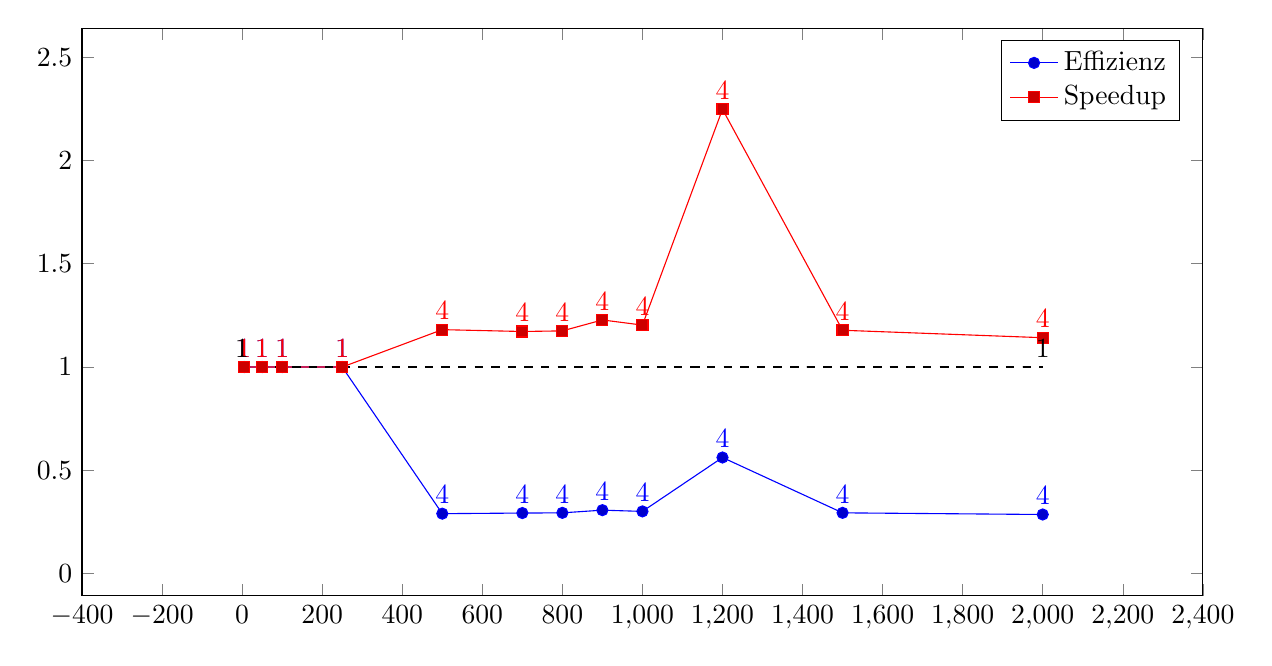
\begin{tikzpicture}
		\begin{axis}[nodes near coords,enlargelimits=0.2,width=450, height=250]

		    \addplot+[
		        point meta=explicit symbolic]
		    coordinates {
		        (5,1) [1]
		        (50,1) [1]
		        (100,1) [1]
		        (250,1) [1]
		        (500,0.29) [4]
		        (700,0.293) [4]
		        (800,0.294) [4]
		        (900,0.307) [4]
		        (1000,0.301) [4]
		        (1200,0.562) [4]
		        (1500,0.294) [4]
		        (2000,0.286) [4]
		    };
		    \addlegendentry{Effizienz}

		    \addplot+[
		        point meta=explicit symbolic]
		    coordinates {
		        (5,1) [1]
		        (50,1) [1]
		        (100,1) [1]
		        (250,1) [1]
		        (500,1.181) [4]
		        (700,1.172) [4]
		        (800,1.175) [4]
		        (900,1.228) [4]
			    (1000,1.203) [4]
			    (1200,2.248) [4]
			    (1500,1.178) [4]
			    (2000,1.142) [4]
			};
		    \addlegendentry{Speedup}

		    \addplot+[
		        smooth,
		        dashed,
		        black,
		        mark=none]
		    coordinates {
		    	(0,1)
		    	(2000,1)
		    };

		\end{axis}
	\end{tikzpicture}
\end{figure}
% subsection dichte (end)